\documentclass[twoside]{article}
\usepackage[utf8]{inputenc}
\usepackage[english]{babel}
\usepackage{amsmath}
\usepackage{graphicx}

\begin{document}
\title{First assignment}
\author{Joaquim Brugués Mora}
\maketitle

{\bf Let $F$ define the map

$$\begin{array}{rccc} F : & [-\pi,\pi] \times [-\pi,\pi] & \longrightarrow & [-\pi,\pi] \times [-\pi,\pi] \\ & \begin{pmatrix} x \\ y \end{pmatrix} & \longmapsto & \begin{pmatrix} x + a \sin(x+y) \\ x+y \end{pmatrix} \end{array} ,$$

where $a$ is a constant, and we take modulo $2\pi$ to ensure the image lies in the square again (this means that the function maps the torus to itself). Study the dynamical system defined by this map.}

\

{\bf 1. Simulate the dynamics taking 100 iterates for each initial condition. Try different initial conditions. Then, modify the code such that the program takes $N$ initial conditions on the $x$-axis. Plot the results.}

We have a MATLAB function {\it map.m} that computes the map for us anytime we need. We use it at the script {\it test1.m}, that generates any number of orbits that the user wishes, with the initial conditions that one gives explicitly. Observe that the code asks for values of $a$ and the number of orbits, but has default values. Anytime this scripts ask for a parameter that takes a default value, the user can just press Enter and the default value will be used. We always take $a=-0.7$ and number of iterates $= 100$.

We runned {\it test1.m}, and took the following five initial conditions (for no particular reason):

$$x_1 = \begin{pmatrix}0.5 \\ 1\end{pmatrix} , x_2 =  \begin{pmatrix} -0.3 \\ 3\end{pmatrix} , x_3 = \begin{pmatrix} 0.1 \\ 2\end{pmatrix} , x_4 = \begin{pmatrix} 0.1 \\ -0.5 \end{pmatrix} , x_5 = \begin{pmatrix} 0.1 \\ 3\end{pmatrix} ,$$

and this gave us the plot

\begin{figure}[!ht]
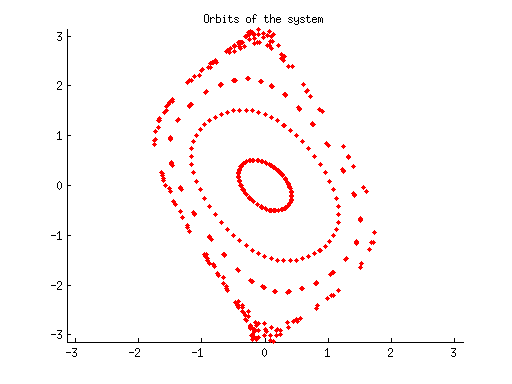
\includegraphics[scale=0.5]{test1.png}
\end{figure}

\

\

\

\

\

\

We also have the script {\it test2.m}, that plots the number of orbits we wish starting at $N$ equidistributed points at the $x$-axis between $-\pi$ and $\pi$. The result taking 200 initial points, for instance, is

\begin{figure}[!ht]
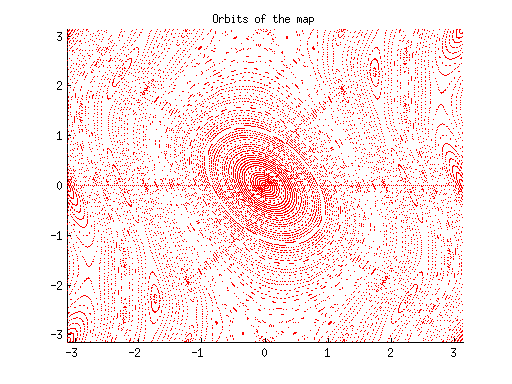
\includegraphics[scale=0.5]{test2.png}
\end{figure}

{\bf 2- Find exact initial condition for a 2-periodic orbit}

We can see that $x_0 = \begin{pmatrix}\pi \\ 0 \end{pmatrix}$ gives a 2-periodic point. This is because

$$F \begin{pmatrix}\pi \\ 0 \end{pmatrix} = \begin{pmatrix}\pi - 0.7 \sin(\pi) \\ \pi \end{pmatrix} =  \begin{pmatrix}\pi \\ \pi \end{pmatrix} ,$$

$$F \begin{pmatrix}\pi \\ \pi \end{pmatrix} = \begin{pmatrix}\pi - 0.7 \sin(2\pi) \\ 2\pi \end{pmatrix} = \begin{pmatrix}\pi \\ 0 \end{pmatrix} .$$

\

{\bf 3. Find approximate initial condition for a 3-periodic orbit.}

We prepared the script {\it zoom.m} to make more detailed plots of the system around certain plots. Using this, and the {\it test2.m}, we can get a detailed picture of the system around the "periodic islands".

For instance, if we take 100 orbits around the point $ \begin{pmatrix} 2.25 \\ 0 \end{pmatrix}$ and a square of size $0.5 \times 0.5$, we get the plot

\begin{figure}[ht]
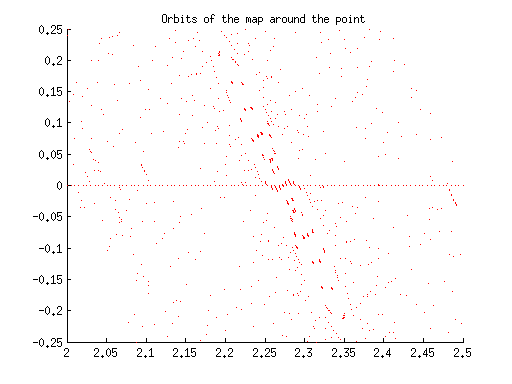
\includegraphics[scale=0.4]{zoom3.png}
\end{figure}

To have a more refined approximations, we prepared the function {\it mapk.m} and the script {\it findPeriods.m}, that allow us to find periodic points via solving the equation

$$F^k(x) - x = 0 ,$$

taking $k=3$ in this case. We need a good initial approximation to ensure that our code converges to a real 3-periodic point, and here is where {\it zoom.m} proves to be useful.

In this case, taking the initial point $x_0 =  \begin{pmatrix} 2.3 \\ 0 \end{pmatrix}$ as suggested by the plot, we find the approximate 3-periodic orbit

$$x_1 =  \begin{pmatrix} 2.272589 \\ 0 \end{pmatrix} , x_2 = F(x_1) =  \begin{pmatrix} 1.738008 \\ 2.272589 \end{pmatrix} , x_3 = F^2(x_1) =  \begin{pmatrix} 2.272589 \\ -2.272589 \end{pmatrix} .$$

\

{\bf 4- Find approximate initial condition for a 4-periodic point.}

Using the same process and codes as before, we get a plot near the 4-periodic island, around the point $\begin{pmatrix} 2 \\ 0 \end{pmatrix}$

\begin{figure}[ht]
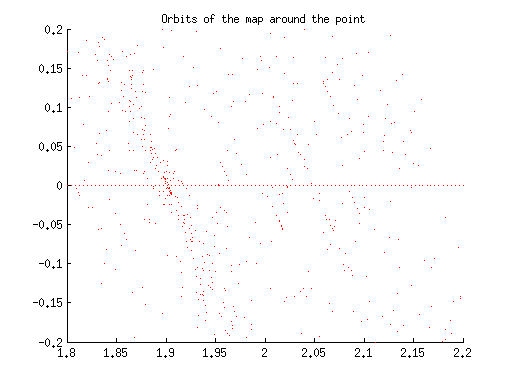
\includegraphics[scale=0.36]{zoom4.png}
\end{figure}

And {\it findPeriods.m} gives us the 4-periodic orbit

$$x_1 = \begin{pmatrix} 1.901797 \\ 0 \end{pmatrix} , x_2 = F(x_1) = \begin{pmatrix}1.239795 \\ 1.901797 \end{pmatrix} ,$$
$$x_3 = F^2(x_1) = \begin{pmatrix} 1.239795 \\ -\pi \end{pmatrix} , x_4 = F^3(x_1) = \begin{pmatrix} 1.901797 \\ -1.901797 \end{pmatrix} .$$

\end{document}